\documentclass[11pt,a4paper]{article}

\usepackage[T1]{fontenc}
\usepackage[utf8]{inputenc}
\usepackage{newtxtext,newtxmath}
\usepackage{microtype}
\usepackage[a4paper,margin=25mm,headheight=14pt]{geometry}
\usepackage{mathtools}
\usepackage{booktabs,array,tabularx,longtable}
\usepackage{enumitem}
\usepackage{xcolor}
\usepackage{tcolorbox}
\usepackage{tikz}
\usetikzlibrary{arrows.meta,positioning,calc}
\usepackage{fancyhdr}
\usepackage{titlesec}
\usepackage{hyperref}
\usepackage{bookmark}

\definecolor{ink}{HTML}{171717}
\definecolor{deepblue}{HTML}{183B66}
\definecolor{teal}{HTML}{1C6B73}
\definecolor{softblue}{HTML}{EEF4FA}
\definecolor{softteal}{HTML}{EDF7F6}
\definecolor{softgray}{HTML}{F4F4F2}
\definecolor{rulegray}{HTML}{C8CDD2}

\hypersetup{
  colorlinks=true,
  linkcolor=deepblue,
  urlcolor=teal,
  citecolor=deepblue,
  pdftitle={Free Numbers Core v1 - Closure Note},
  pdfauthor={Residual Chart Lab}
}

\pagestyle{fancy}
\fancyhf{}
\fancyhead[L]{\small\textsc{Free Numbers Core v1}}
\fancyhead[R]{\small\textsc{Closure Note}}
\fancyfoot[C]{\small\thepage}
\renewcommand{\headrulewidth}{0.4pt}
\renewcommand{\footrulewidth}{0pt}

\titleformat{\section}
  {\Large\bfseries\color{deepblue}}
  {\thesection}{0.7em}{}
\titleformat{\subsection}
  {\large\bfseries\color{teal}}
  {\thesubsection}{0.7em}{}

\setlist[itemize]{leftmargin=1.6em,itemsep=0.25em,topsep=0.4em}
\setlist[enumerate]{leftmargin=1.8em,itemsep=0.3em,topsep=0.4em}
\setlength{\parindent}{0pt}
\setlength{\parskip}{0.55em}
\setlength{\emergencystretch}{2em}

\newtcolorbox{theorembox}[1][]{
  colback=softblue,
  colframe=deepblue,
  boxrule=0.7pt,
  arc=1.5mm,
  left=3mm,right=3mm,top=2.5mm,bottom=2.5mm,
  title=#1,
  fonttitle=\bfseries
}

\newtcolorbox{resultbox}[1][]{
  colback=softteal,
  colframe=teal,
  boxrule=0.7pt,
  arc=1.5mm,
  left=3mm,right=3mm,top=2.5mm,bottom=2.5mm,
  title=#1,
  fonttitle=\bfseries
}

\newtcolorbox{scopebox}[1][]{
  colback=softgray,
  colframe=rulegray,
  boxrule=0.6pt,
  arc=1.5mm,
  left=3mm,right=3mm,top=2.5mm,bottom=2.5mm,
  title=#1,
  fonttitle=\bfseries
}

\newcommand{\Hq}{\mathbb H}
\newcommand{\RR}{\mathbb R}
\newcommand{\Fn}{\mathfrak F_{\mathrm{v1}}}
\newcommand{\An}{\mathfrak A}
\newcommand{\tensor}{\mathbin{|}}
\newcommand{\st}{\star}
\newcommand{\Img}{\operatorname{im}}
\newcommand{\Hom}{\operatorname{Hom}}
\newcommand{\degf}{\operatorname{deg}}

\begin{document}

\begin{titlepage}
\thispagestyle{empty}
\centering
\vspace*{18mm}

{\Huge\bfseries\color{deepblue} Free Numbers Core v1\par}
\vspace{4mm}
{\LARGE Quaternionic Exact-Response Core\par}
\vspace{4mm}
{\large Closure Note\par}

\vspace{18mm}

\begin{tcolorbox}[
  width=0.88\textwidth,
  colback=softblue,
  colframe=deepblue,
  boxrule=0.9pt,
  arc=2mm,
  left=5mm,right=5mm,top=6mm,bottom=6mm
]
\centering
\[
\boxed{
\Fn
=
\left(
\An,
\st,
1,
\degf,
(\mu_n)_{n\ge0},
\mathcal P,
(F_d^{(n)})
\right)
}
\]
\end{tcolorbox}

\vfill

{\large Residual Chart Lab\par}
\vspace{2mm}
{\normalsize July 2026\par}

\vspace{15mm}
{\small
A complete finite-grade realization with non-collapsing compression,\par
contextual re-observability, recursive decoding, and uniform composition.\par
}
\end{titlepage}

\tableofcontents
\newpage

\section*{Abstract}
\addcontentsline{toc}{section}{Abstract}

This note closes the first standalone Free Numbers core. The closed object is not a universal classification of every possible realization; it is the first exact, finite-grade, compositional model in which compression-hidden structure is retained and recovered.

Let
\[
V=\operatorname{Im}\Hq,
\qquad
B_n=V^{\otimes n},
\]
with reversed quaternionic compression. The canonical all-gap response
\[
A_n:B_n\longrightarrow \Hom(V^{\otimes(n-1)},\Hq)
\]
is injective for every finite grade. A single twelve-dimensional local decoder, with determinant
\[
\det\Theta=256,
\]
peels off one outer boundary letter at a time without information loss. Exact response coordinates compose by an ordered bridge product, producing a unital associative graded algebra. Lower-depth observations retain their independent role as a spectrum of first-detection depth.

\begin{theorembox}[Closure verdict]
\[
\boxed{
\text{Free Numbers Core v1}
=
\text{Quaternionic Exact-Response Core}
}
\]
The reconstruction and composition problem is closed. The residual-depth spectrum remains open.
\end{theorembox}

\section{The closed package}

The Core v1 package is
\[
\boxed{
\Fn
=
\left(
\An,
\st,
1,
\degf,
(\mu_n)_{n\ge0},
\mathcal P,
(F_d^{(n)})
\right).
}
\]

Its components have distinct roles:

\begin{itemize}
\item $\An=\bigoplus_{n\ge0}\mathfrak A_n$ is the exact-response carrier.
\item $\st$ is the ordered, cross-boundary composition law.
\item $1\in\mathfrak A_0$ is the empty-boundary unit.
\item $\degf$ preserves structural length.
\item $\mu_n$ recovers the compressed quaternionic value.
\item $\mathcal P$ is the admitted family of insertion probes.
\item $F_d^{(n)}$ is the residual-depth filtration.
\end{itemize}

\begin{scopebox}[Model-first closure]
The phrase ``complete core'' means complete for this exact quaternionic realization. It does not mean that every possible Free Numbers model must be quaternionic, nor that the depth spectrum has been fully classified.
\end{scopebox}

\section{Graded representatives and compression}

Let
\[
B_0=\RR\mathbf 1,
\qquad
B_n=V^{\otimes n}\quad(n\ge1),
\]
where $\mathbf 1$ is the empty boundary word. The representative carrier is the tensor algebra
\[
T(V)=\bigoplus_{n\ge0}B_n.
\]
Composition is concatenation,
\[
\Vert:B_m\times B_n\longrightarrow B_{m+n},
\]
which is strictly associative and satisfies
\[
\degf(x\Vert y)=\degf x+\degf y.
\]

For a pure boundary word,
\[
\boxed{
 m_n(a_1\tensor\cdots\tensor a_n)=a_n\cdots a_1.
}
\]
At grade zero, $m_0(\lambda\mathbf1)=\lambda$.

Compression is deliberately many-to-one. Equality of values,
\[
m_n(x)=m_n(y),
\]
does not imply equality of Free Numbers. The compression fiber is retained inside the exact state rather than discarded.

\section{Canonical all-gap response}

For $n=1$, set $A_1(a)=a$. For $n\ge2$, define
\[
\boxed{
A_n(a_1\tensor\cdots\tensor a_n)(d_1,\ldots,d_{n-1})
=
a_nd_{n-1}a_{n-1}\cdots d_1a_1.
}
\]

This inserts one probe into every original internal gap and then applies reversed compression. The exact-response space is
\[
\mathfrak A_n:=\Img A_n
\subseteq
\Hom(V^{\otimes(n-1)},\Hq),
\qquad
\mathfrak A_0:=\RR.
\]

The low-grade vertical-response theorem is recovered as the highest-spin restriction:
\[
A_n(S)=(-2)^{n-1}C_S,
\qquad
S\in S^n_0V.
\]

\section{The local decoder}

The entire all-grade theorem is controlled by one local map:
\[
\Theta:V\otimes\Hq\longrightarrow\Hom(V,\Hq),
\]
\[
\boxed{
\Theta\!\left(\sum_{a=1}^3e_a\otimes h_a\right)(d)
=
\sum_{a=1}^3e_a d h_a.
}
\]

Both domain and codomain have real dimension twelve. More importantly, the inverse is explicit. For $F\in\Hom(V,\Hq)$,
\[
\boxed{
h_a
=
\frac12
\sum_{b,c=1}^3
\varepsilon_{abc}\,e_bF(e_c).
}
\]
Then
\[
F(d)=\sum_{a=1}^3e_a d h_a.
\]

\begin{resultbox}[The local gate has no kernel]
\[
\boxed{
\Theta\text{ is an isomorphism},
\qquad
\det\Theta=256.
}
\]
The outermost boundary layer can therefore be removed without loss.
\end{resultbox}

\subsection{The peeling ladder}

Every $x\in B_n$ has a unique expansion
\[
x=\sum_{a=1}^3x_a\tensor e_a,
\qquad
x_a\in B_{n-1}.
\]
For $\mathbf d=(d_1,\ldots,d_{n-2})$,
\[
A_n(x)(\mathbf d,d)
=
\sum_{a=1}^3e_a d\,A_{n-1}(x_a)(\mathbf d).
\]
Applying $\Theta^{-1}$ to the final-variable slice recovers all three functions $A_{n-1}(x_a)$ exactly.

\begin{center}
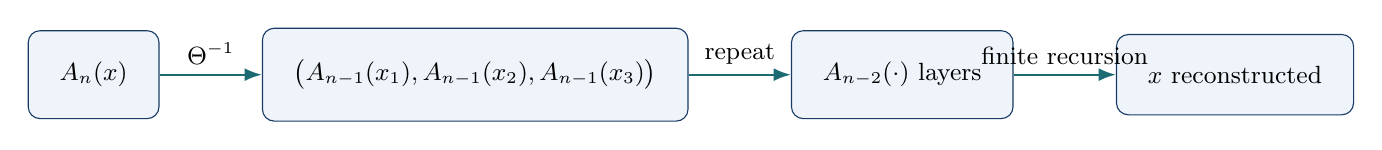
\begin{tikzpicture}[
  node distance=10mm and 13mm,
  every node/.style={font=\small},
  box/.style={draw=deepblue,rounded corners=1.5mm,fill=softblue,inner sep=4mm,align=center},
  arr/.style={-{Latex[length=2.2mm]},thick,draw=teal}
]
\node[box] (an) {$A_n(x)$};
\node[box,right=of an] (split) {$\bigl(A_{n-1}(x_1),A_{n-1}(x_2),A_{n-1}(x_3)\bigr)$};
\node[box,right=of split] (next) {$A_{n-2}(\cdot)$ layers};
\node[box,right=of next] (x) {$x$ reconstructed};
\draw[arr] (an) -- node[above] {$\Theta^{-1}$} (split);
\draw[arr] (split) -- node[above] {repeat} (next);
\draw[arr] (next) -- node[above] {finite recursion} (x);
\end{tikzpicture}
\end{center}

The same twelve-dimensional gate is reused at every rung. No global search through the full tensor basis is required.

\section{All-grade reconstruction}

\begin{theorembox}[All-Grade Reconstruction Theorem]
For every finite $n\ge0$,
\[
\boxed{
A_n:B_n\xrightarrow{\cong}\mathfrak A_n.
}
\]
Equivalently,
\[
\boxed{
A_n(x)=A_n(y)
\iff
x=y.
}
\]
\end{theorembox}

The proof is inductive. If $A_n(x)=0$, the final-variable slice is killed by $\Theta$. Since $\Theta$ is injective, each $A_{n-1}(x_a)$ vanishes. The induction hypothesis gives $x_a=0$ for every $a$, hence $x=0$.

Consequently,
\[
\operatorname{rank}A_n=3^n,
\qquad
\dim\mathfrak A_n=3^n.
\]
The ambient multilinear space has dimension $4\cdot3^{n-1}$, so the admissible response space is a proper structured subspace of codimension $3^{n-1}$.

\begin{resultbox}[Finite visibility]
\[
\boxed{
A_n(x)=0\Longrightarrow x=0,
\qquad
F_n^{\infty}=0.
}
\]
Every nonzero finite representative becomes visible by depth at most $n-1$.
\end{resultbox}

\section{Uniform composition}

Let $x\in B_m$ and $y\in B_n$. Write the internal probes of $x$ as $\mathbf d$, the bridge probe as $\delta$, and the internal probes of $y$ as $\mathbf e$. Then
\[
\boxed{
A_{m+n}(x\Vert y)(\mathbf d,\delta,\mathbf e)
=
A_n(y)(\mathbf e)\,\delta\,A_m(x)(\mathbf d).
}
\]

For $F\in\mathfrak A_m$ and $G\in\mathfrak A_n$, define
\[
\boxed{
(F\st G)(\mathbf d,\delta,\mathbf e)
:=
G(\mathbf e)\,\delta\,F(\mathbf d).
}
\]
The order is structural: the right factor appears on the left under reversed quaternionic compression.

Thus
\[
\boxed{
A_m(x)\st A_n(y)=A_{m+n}(x\Vert y).
}
\]
For grade zero,
\[
\lambda\st F=F\st\lambda=\lambda F.
\]

\begin{theorembox}[Exact-response algebra]
\[
\boxed{
(\An,\st,1)
\text{ is a unital associative graded real algebra.}
}
\]
Moreover,
\[
\boxed{
A:T(V)\xrightarrow{\cong}\An
}
\]
is a graded algebra isomorphism.
\end{theorembox}

The isomorphism does not empty the theory of content. Free Numbers Core v1 retains distinguished compression maps, zero fibers, probe families, and depth filtrations in addition to the algebraic carrier.

\section{Active zero states and residual collision}

Transport compression to exact-response coordinates:
\[
\mu_n:=m_n\circ A_n^{-1}:
\mathfrak A_n\longrightarrow\Hq.
\]
The zero fiber is
\[
Z_n:=\ker\mu_n.
\]
An active zero state is a nonzero $F\in Z_n$.

At grade two,
\[
Z_2\cong S^2_0V,
\qquad
A_2(S)=-2C_S.
\]
Thus a state can be completely zero under compression while remaining nonzero under contextual response.

At grade four, let $S,T\in S^2_0V$ be nonzero pure residuals. Then
\[
m_4(S\Vert T)=0,
\]
and every depth-one response vanishes. Yet the middle depth-two response is
\[
\boxed{
D_{13}(S\Vert T)(d_1,d_2)
=
4T(d_2)S(d_1)
\ne0.
}
\]
Hence
\[
\boxed{
\delta(S\Vert T)=2.
}
\]
Two zero-valued factors compose to a zero-valued, depth-one-invisible state whose internal collision is necessarily visible at depth two.

\section{Depth splitting and higher coherence}

The length-four factor-origin decomposition is
\[
B_4\cong VV\oplus VR\oplus RV\oplus RR,
\]
where $V$ denotes the value sector and $R=S^2_0V$ the residual sector. The exact remaining-kernel table is:

\begin{center}
\renewcommand{\arraystretch}{1.18}
\begin{tabular}{lrrrrr}
\toprule
sector & dimension & $F_0$ & $F_1$ & $F_2$ & $F_3$\\
\midrule
$VV$ & 16 & 12 & 0 & 0 & 0\\
$VR$ & 20 & 20 & 12 & 0 & 0\\
$RV$ & 20 & 20 & 12 & 0 & 0\\
$RR$ & 25 & 25 & 25 & 9 & 0\\
\midrule
total & 81 & 77 & 49 & 9 & 0\\
\bottomrule
\end{tabular}
\end{center}

This resolves the previously unexplained split of six spin-two copies:
\[
6V_2
=
1_{VV}+2_{VR}+2_{RV}+1_{RR}.
\]
Three copies are first detected at depth one and three at depth two. The split is not random behavior inside a spin label; it is the visible trace of distinct factor origins and cross-boundary channels.

Inside
\[
RR=S^2_0V\otimes S^2_0V,
\]
the map $D_{13}$ has rank sixteen. Compression and every depth-one response
vanish on $RR$, while $D_{13}$ is the only depth-two component that can remain.
Consequently,
\[
\ker(D_{13}|_{RR})=F_2^{(4)}\cap RR.
\]
The independently verified length-four equality
\[
F_2^{(4)}=S^4_0V
\]
and the inclusion $S^4_0V\subset RR$ give
\[
\boxed{
\ker(D_{13}|_{RR})=S^4_0V=V_4.
}
\]
The rank count $25-16=9=\dim V_4$ is a consistency check, not the sole
identification argument. The nine-dimensional survivor contains no nonzero
decomposable tensor $S\otimes T$. It consists of coherent superpositions whose
individual depth-two responses cancel exactly.

At depth three,
\[
A_4(R)=-8C_R
\qquad(R\in S^4_0V),
\]
so the remaining coherence is fully detected.

\begin{resultbox}[Higher coherence]
The depth-three survivor is not a single residual pair. It is a structured superposition of residual pairs whose depth-two collision responses cancel, while the combined state remains nonzero and reappears as a harmonic fourth-order tensor.
\end{resultbox}

\section{Residual-depth filtration}

Let $D_n^{\le d}$ be the combined response profile through depth $d$. Define
\[
F_d^{(n)}:=\ker D_n^{\le d}.
\]
Then
\[
F_0^{(n)}\supseteq F_1^{(n)}\supseteq\cdots\supseteq F_{n-1}^{(n)}=0.
\]
For a nonzero state,
\[
\delta(x)
=
\min\{d:D_n^{\le d}(x)\ne0\}.
\]

What is closed is the termination bound
\[
\boxed{
\delta(x)\le n-1
\qquad(x\in B_n\setminus\{0\}).
}
\]
What remains open is the classification of the intermediate quotients
\[
F_{d-1}^{(n)}/F_d^{(n)}
\]
by spin, multiplicity, factor origin, and probe depth.

\section{Capability closure}

\renewcommand{\arraystretch}{1.22}
\begin{longtable}{>{\bfseries}p{13mm}p{34mm}p{95mm}}
\toprule
ID & capability & Core v1 witness\\
\midrule
\endhead
C1 & History distinction & States with equal compressed value may have distinct exact responses.\\
C2 & Non-collapsing compression & Compression fibers remain inside $\mathfrak A_n$ and never define equality.\\
C3 & Contextual re-observability & Every nonzero finite state is recovered by an admitted all-gap context.\\
C4 & Residual depth & $F_d^{(n)}$ and $\delta(x)$ are defined, with termination by depth $n-1$.\\
C5 & Composition & Exact coordinates compose by the bridge product $\st$.\\
C6 & Closure with remainder & $\mu_n(F)$ and all information omitted by it coexist in $F$.\\
C7 & No retrospective deletion & Grade is retained and additive; Core v1 has no deletion operation.\\
C8 & Standalone equality & $A_n(x)=A_n(y)$ is finite, exact, and composition-compatible.\\
C9 & Finite observability & $A_n$ is a complete finite certificate with an explicit decoder.\\
C10 & Quaternionic recovery & $\mu_n$ recovers $\Hq$ value without identifying the full state with $\Hq$.\\
\bottomrule
\end{longtable}

\begin{theorembox}[Capability Closure Theorem]
\[
\boxed{
\text{Free Numbers Core v1 satisfies C1--C10.}
}
\]
All primitives and proofs are stated without the Time Engine, future endpoints, consciousness, ethics, Y-axis terminology, registry machinery, or normalization machinery.
\end{theorembox}

\section{Core Closure Theorem}

\begin{theorembox}[Free Numbers Core v1]
Let
\[
\Fn
=
\left(
\An,
\st,
1,
\degf,
(\mu_n)_{n\ge0},
\mathcal P,
(F_d^{(n)})
\right).
\]
Then:
\begin{enumerate}
\item $\An$ is a unital associative graded real algebra;
\item every finite representative has a unique exact response coordinate;
\item the coordinate is recursively decoded without information loss;
\item every finite nonzero state is visible by depth at most $n-1$;
\item compression is non-injective but does not destroy the retained state;
\item zero-valued nonzero states exist and compose nontrivially;
\item exact coordinates compose uniformly by $\st$;
\item exact equality is a composition-compatible standalone equality;
\item quaternionic value is recovered without confining the full object to $\Hq$;
\item C1--C10 hold independently of the Residual Chart OS and originating interpretation.
\end{enumerate}
Therefore,
\[
\boxed{
\Fn
\text{ is a complete standalone Free Numbers core.}
}
\]
\end{theorembox}

This closure is model-first rather than universal:
\[
\boxed{
\text{first complete core}
\ne
\text{final classification of all cores}.
}
\]

\newpage
\section{Stopping rule}

The first reconstruction cycle stops here.

\begin{resultbox}[Closed question]
\centering
Can every finite state be represented, reconstructed, compared, and composed\\
without losing compression-hidden structure?
\end{resultbox}

\begin{center}
\Large\bfseries Yes.
\end{center}

\begin{scopebox}[Open question]
\centering
How is that structure distributed across the residual-depth spectrum?
\end{scopebox}

That is the next research program. Further $n=5,6,\ldots$ spin-depth tables belong to the open mine, not to the completion requirement of Core v1.

\vfill
\begin{tcolorbox}[
  colback=deepblue,
  colframe=deepblue,
  boxrule=0pt,
  arc=2mm,
  left=5mm,right=5mm,top=6mm,bottom=6mm
]
\centering
{\Large\bfseries\color{white} Free Numbers Core v1 is closed.\par}
\vspace{3mm}
{\large\color{white} The mine remains open. The foundation does not.\par}
\end{tcolorbox}

\end{document}
